\section{Motivation for Demand Management}
\label{strategies}
We measured the power consumption of Sequoia, the world's third fastest supercomputer at 17.1 petaflops, hosted at LLNL. Sequoia is a BlueGene/Q design-based system with 98,304 16-core PowerPC A2 compute nodes that has a power rating of 7.9 MW. The data from Sequoia was collected at three-minute intervals over three days and the results can be seen from Figure \ref{fig:seq}. Information about the workload being executed was not made available. The y-axis is the power consumed, and the x-axis represents the time samples.  As can be noted from this figure, fluctuations of a few megawatts are fairly common. Some of these fluctuations may be related to maintenance cycles and could be scheduled or forecasted. However, there are other times where the fluctuations are not scheduled in advance and may occur as a result of the workload that is executing on the supercomputer. 

\begin{figure}
\begin{center}
\frame{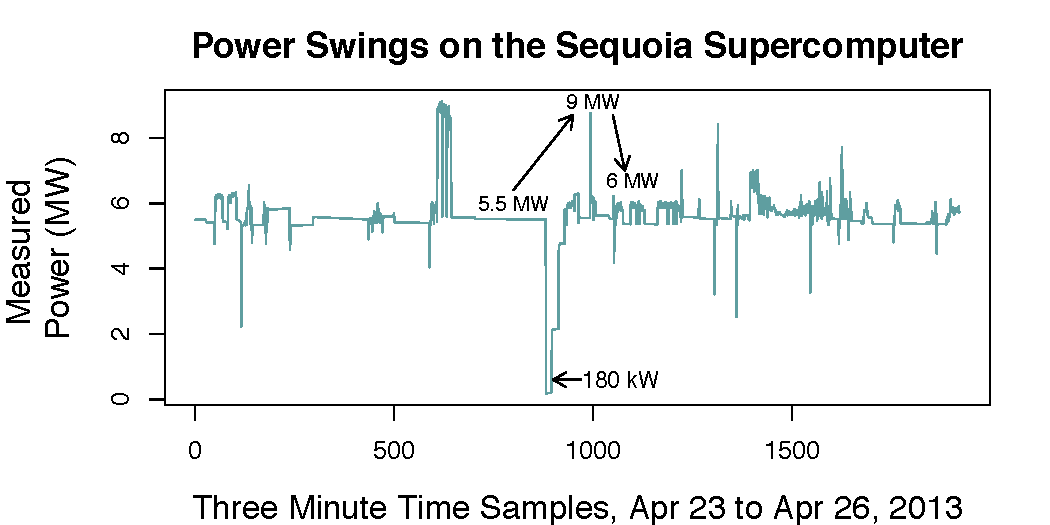
\includegraphics[scale=0.55]{figs/seq.pdf}}
\caption{Sequoia Supercomputer Power Swings}
\label{fig:seq}
\end{center}
\end{figure}

\begin{figure}
\begin{center}
\frame{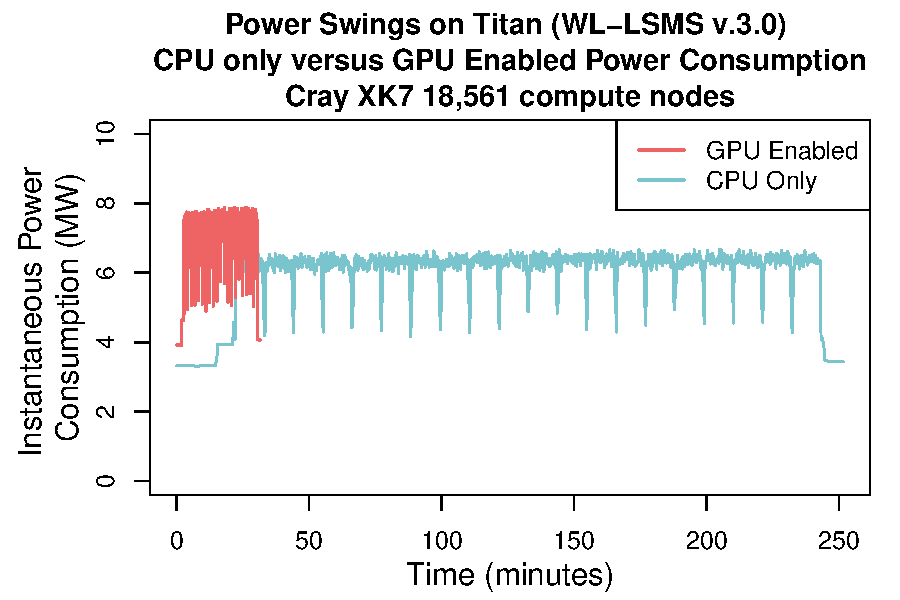
\includegraphics[scale=0.55]{figs/ORNLData.pdf}}
\caption{Titan Supercomputer Power Swings}
\label{fig:titan}
\end{center}
\end{figure}

We observe similar trends with data from Titan, which is the world's second-fastest supercomputer hosted at ORNL. Titan is a 17.6 petaflop system with a power rating of 8.2 MW. It comprises of 18,688 16-core AMD Opteron 6274 compute nodes, and each compute node has a NVIDIA Tesla K20X GPU. Figure \ref{fig:titan} shows data gathered from identical WL-LSMS executions on the Titan supercomputer. WL-LSMS is a benchmark that performs thermodynamic calculations  \cite{WLLSMS}. The graph in Figure \ref{fig:titan} has instantaneous power in MW on the y-axis and the benchmark execution time on the x-axis. The data is reported for a CPU-only run as well as a GPU-enabled run. The power samples for the CPU-only run were collected every 8 minutes, where as the samples for the GPU-enabled run were reported every second. The red line represents the GPU-enabled run and the blue line represents the CPU-only run.  As can be noted from this data, substantial power swings are observed on Titan, both in the case of CPU-only as well as GPU-enabled runs. 

The energy efficiency improves by about seven times when the GPU is enabled as the application runs significantly faster. Note that the power swings observed here are a result of the ensemble runs of WL-LSMS. They occur when a new set of calculations is being initiated and there is a pause between the compute-intensive work phases. This trend is observed for both the GPU-enabled and the CPU-only runs. Also, the peak power and power fluctuations are only slightly different with the GPU-enabled run than they are with the CPU-only run. Peak power increased by about one megawatt with the GPU-enabled run. The net effect is that less energy is used to get the same work done in the GPU-enabled case, but with slightly higher power draw and potentially higher power variability.

Both these datasets clearly indicate that power fluctuations occur in real production systems, and this can affect the reliability of the ESP grid. It is thus imperative to understand how such variable power demands can be managed better. In this context, demand management (DM) is one approach to mitigate the consequences of these power fluctuations that promotes a tighter relationship between ESPs and SCs. %SCs can forecast and communicate with their ESPs more often to discuss and address such issues. 

\section{Demand Management}
\label{dm}
Demand Management covers strategies, programs and methods that SCs and ESPs can employ to ensure grid reliability. We define \emph{strategies} as power management techniques used by SCs to manage power and provide load flexibility. Strategies may or may not improve energy efficiency. For example, \emph{Load Migration} is a strategy that SCs may use in response to an ESP's request, and while it helps manage power effectively, it does not impact the energy efficiency of the site. On the other hand, \emph{fine-grained power management} techniques, such as using node-level power capping, or better job scheduling algorithms are likely to improve energy efficiency but may not be as useful in response to an ESP request. Almost all sites employ some power management strategies, especially the ones involving lighting, temperature, cooling, fine-grain power management and job scheduling. 

\emph{Programs} are incentives offered by ESPs to their customers and to SCs in order to motivate them to help balance the electrical grid and perform power managment. Common examples include peak shedding, peak shifting and dynamic pricing. Peak shedding describes the action where SCs (or consumers) reduce their electricity consumption in response to a request from the ESP. The reduction in electricity consumption does not lead to an increase in consumption at a later point in time. Peak shifting, on the other hand, moves load from one time slot to another, in response to a request from the ESP. Lastly, dynamic pricing is a mechanism used by the ESP to incentivize an increase or decrease in consumption by varying the price of electricity over time.

\emph{Methods} are used by the ESPs to balance the electrical grid in the transmission and distribution phases. Examples of methods include regulation, frequency response, grid scale storage. %and use of renewable sources of energy. 

Another important aspect of DM is the wider acceptance of renewable sources of energy. In the current electricity mix, the benefits of \emph{demand forecasting} (that is, predicting the amount of power required by an SC for a certain period of time) by the SCs and their communication with their ESPs for better capacity planning and electricity purchase negotiations have been shown. Such benefits can be exercised with active DM actions within a forecasted power band as described above. With increasing variable renewable generation in the electricity mix, more granular demand forecasting by the SCs can help ESPs to identify and plan for grid impacts during over- and under-generation conditions. 